\appendix

\chapter{Portal Screenshots}
\label{app:screenshots}

This appendix collects additional screenshots of the Water Data Platform
frontend portal that complement the in-text figures in
Section~\ref{sec:impl-frontend}.

\begin{figure}[ht]
  \centering
  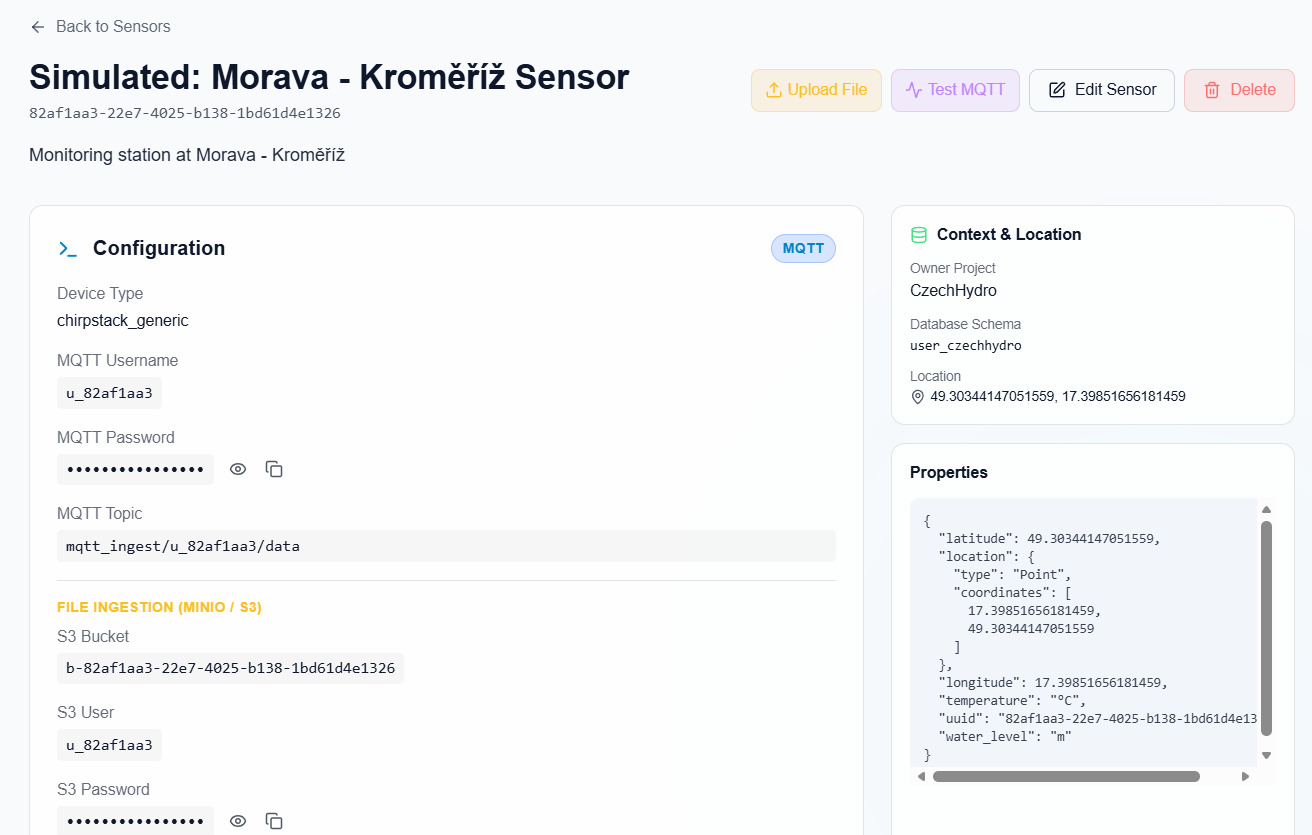
\includegraphics[width=0.95\textwidth]{figures/screenshot-sensor-detail.png}
  \caption{SMS-level sensor detail for a Morava river monitoring station.
           The Configuration panel shows the MQTT credentials, topic, and
           MinIO/S3 bucket for file ingestion. The Context \& Location
           panel displays the owning project, database schema, coordinates,
           and the raw Thing properties JSON.}
  \label{fig:screenshot-sensor-detail-sms}
\end{figure}

\begin{figure}[ht]
  \centering
  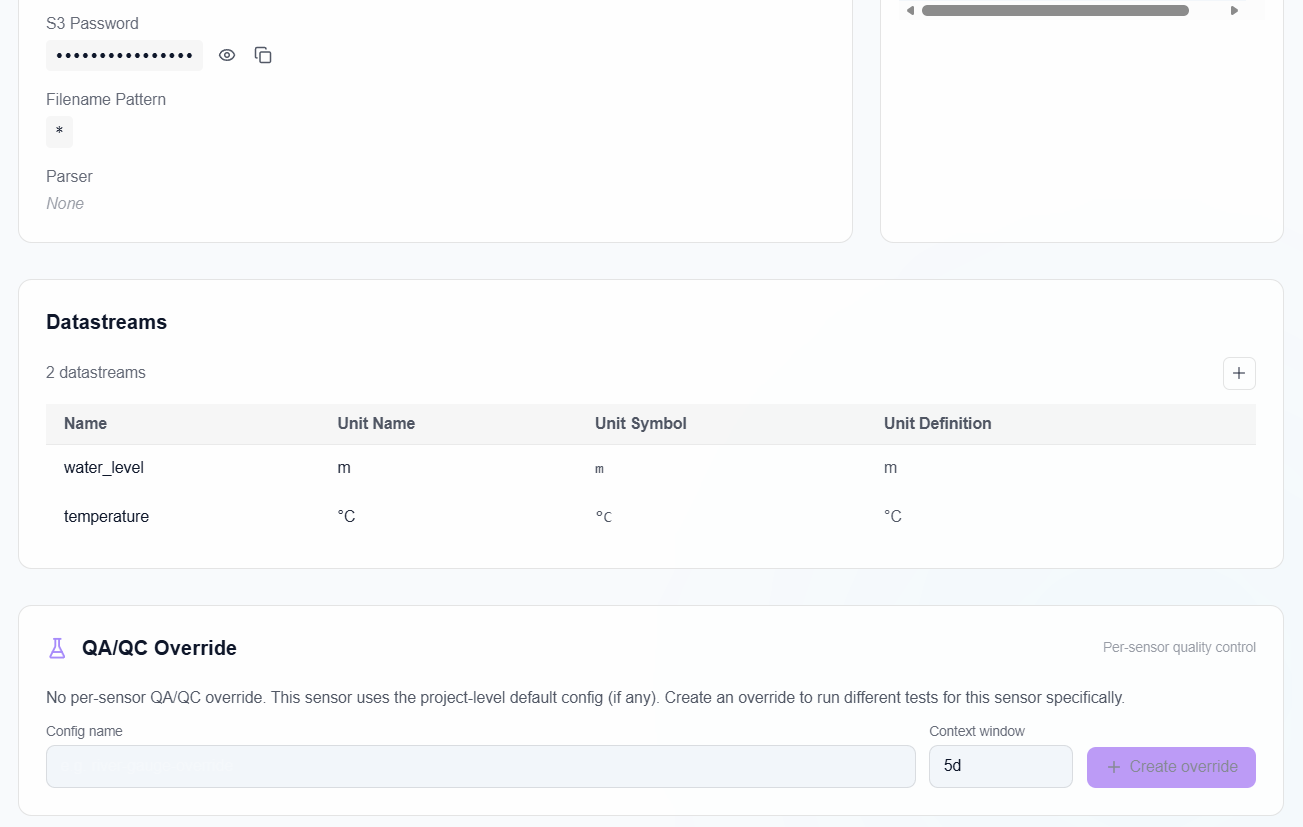
\includegraphics[width=0.95\textwidth]{figures/screenshot-sensor-detail-2.png}
  \caption{SMS-level sensor detail (continued). The Datastreams section
           lists the configured datastreams with their unit names, symbols,
           and definitions. The QA/QC Override section at the bottom allows
           creating a per-sensor quality-control override that replaces the
           project-level default configuration.}
  \label{fig:screenshot-sensor-detail-sms-2}
\end{figure}

\begin{figure}[ht]
  \centering
  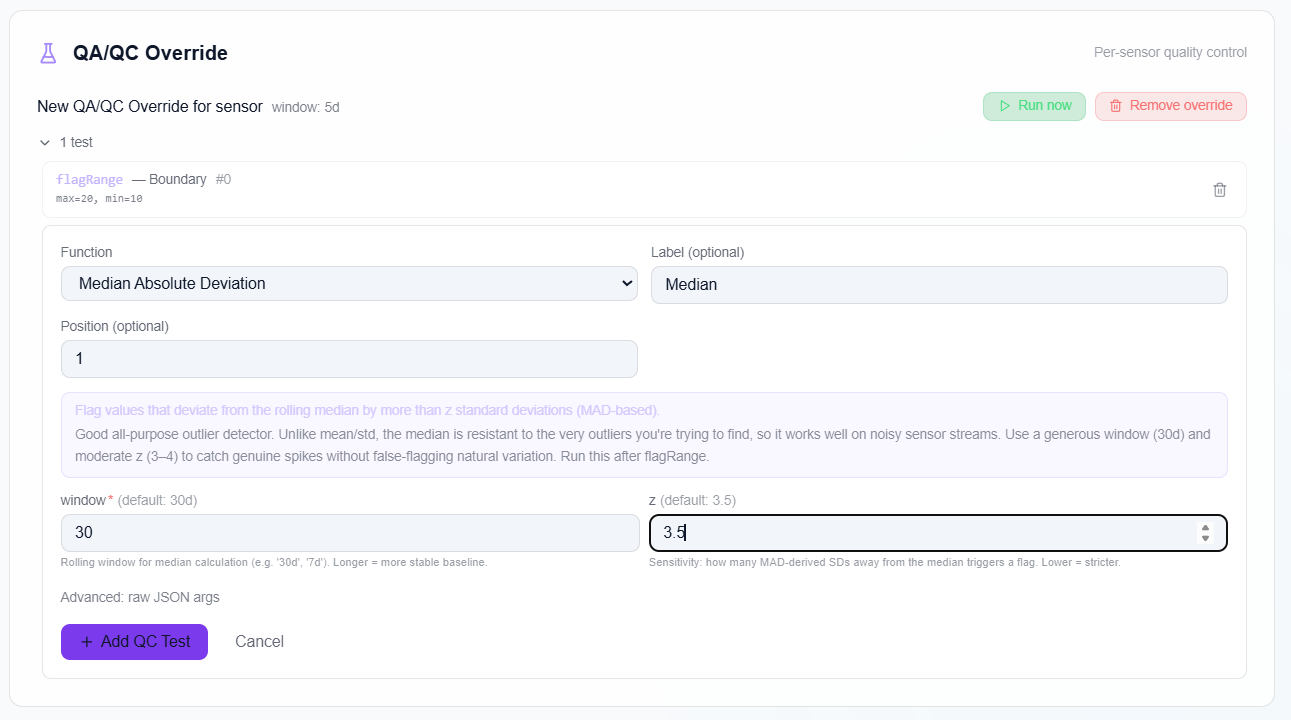
\includegraphics[width=0.95\textwidth]{figures/screenshot-qaqc.png}
  \caption{QA/QC override configuration for a sensor. An existing
           \texttt{flagRange} boundary test is shown at the top. Below it,
           a Median Absolute Deviation test is being added with a 30-day
           rolling window and $z = 3.5$ sensitivity threshold. The
           explanatory text panel describes how each test function works.}
  \label{fig:screenshot-qaqc}
\end{figure}

\begin{figure}[ht]
  \centering
  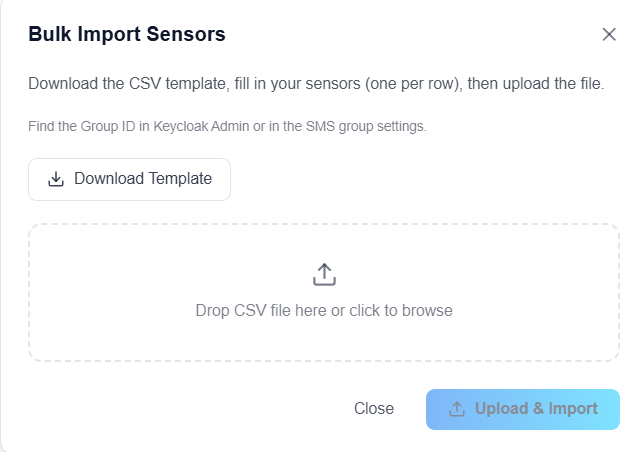
\includegraphics[width=0.6\textwidth]{figures/screenshot-batch-import.png}
  \caption{Bulk Import Sensors dialog. A CSV template can be downloaded,
           filled with sensor definitions (one per row), and uploaded via
           drag-and-drop. The Group~ID links each sensor to a Keycloak
           group.}
  \label{fig:screenshot-batch-import}
\end{figure}

\begin{figure}[ht]
  \centering
  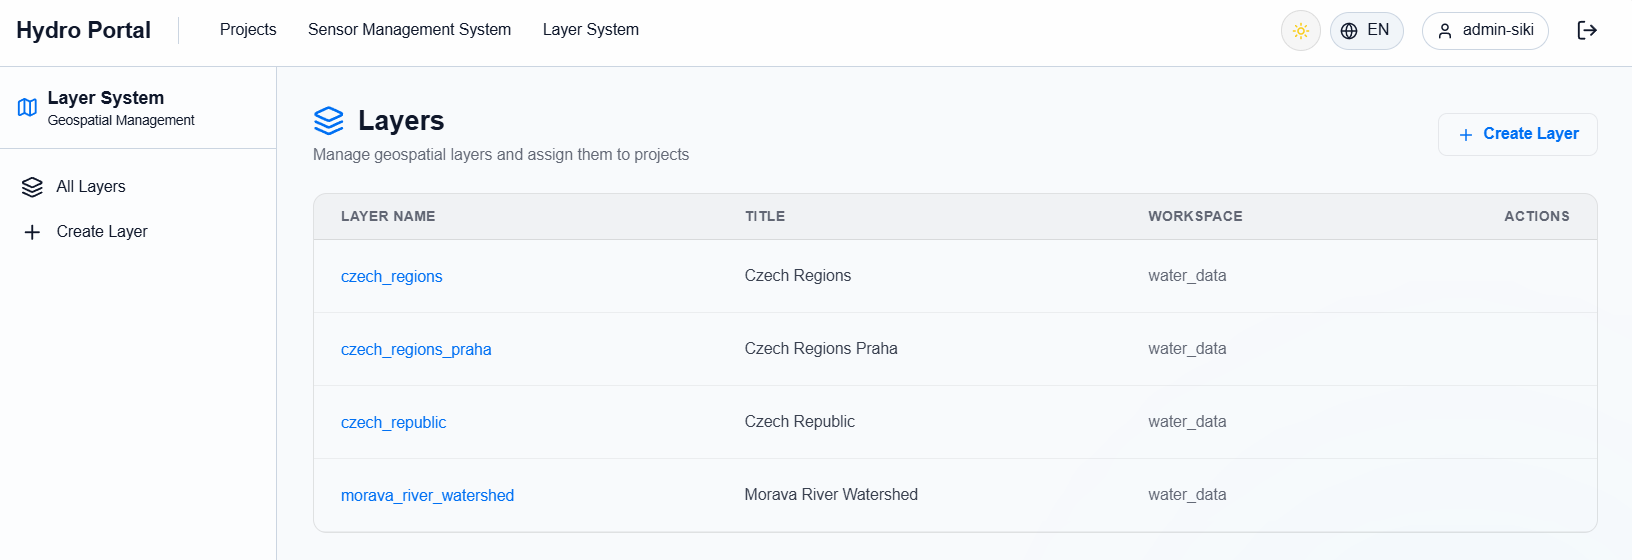
\includegraphics[width=0.95\textwidth]{figures/screenshot-layers.png}
  \caption{Layer System management page listing GeoServer WMS layers.
           Each row shows the layer name, human-readable title, and
           GeoServer workspace. The sidebar provides navigation to the
           full layer list and the layer creation form.}
  \label{fig:screenshot-layers}
\end{figure}

\begin{figure}[ht]
  \centering
  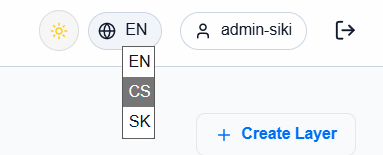
\includegraphics[width=0.35\textwidth]{figures/screenshot-i18n.png}
  \caption{Language switcher dropdown in the application header showing
           the three supported locales: English~(EN), Czech~(CS), and
           Slovak~(SK). The selected locale is persisted in
           \texttt{localStorage}.}
  \label{fig:screenshot-i18n}
\end{figure}
